%%%%%%%%%%%%%%%%%%%%%%%%%%%%%%%%%%%%%%%%%%%%%%%%%%%%%%%%%%%%%%%%%%%%%%
% LaTeX Example: Project Report
%
% Source: http://www.howtotex.com
%
% Feel free to distribute this example, but please keep the referral
% to howtotex.com
% Date: March 2011 
% 
%%%%%%%%%%%%%%%%%%%%%%%%%%%%%%%%%%%%%%%%%%%%%%%%%%%%%%%%%%%%%%%%%%%%%%

%%% Preamble
\documentclass[paper=a4, fontsize=11pt]{scrartcl}
\usepackage[T1]{fontenc}
\usepackage{fourier}
\usepackage[english]{babel}								% English language/hyphenation
\usepackage[protrusion=true,expansion=true]{microtype}	
\usepackage{amsmath,amsfonts,amsthm} 					% Math packages
\usepackage[pdftex]{graphicx}
\usepackage{float}
\graphicspath{{fig/}}
\usepackage{url}
\usepackage[linesnumbered, ruled]{algorithm2e}          % Algorithm pseudo code formatting
\usepackage[titletoc,title]{appendix}
\usepackage{subcaption}
\usepackage{listings}                                   % Code formatting
\usepackage[margin=1in]{geometry}                       % Change the default margins

%%% Custom sectioning
\usepackage{sectsty}
\allsectionsfont{\normalfont\scshape}

%%% Custom headers/footers (fancyhdr package)
\usepackage{fancyhdr}
\pagestyle{fancyplain}
\fancyhead{}							% No page header
\fancyfoot[L]{}							% Empty 
\fancyfoot[C]{}							% Empty
\fancyfoot[R]{\thepage}					% Pagenumbering
\renewcommand{\headrulewidth}{0pt}		% Remove header underlines
\renewcommand{\footrulewidth}{0pt}		% Remove footer underlines
\setlength{\headheight}{13.6pt}

%%% Equation and float numbering
\numberwithin{equation}{section}		% Equationnumbering: section.eq#
\numberwithin{figure}{section}			% Figurenumbering: section.fig#
\numberwithin{table}{section}		    % Tablenumbering: section.tab#

%%% Maketitle metadata
\newcommand{\horrule}[1]{\rule{\linewidth}{#1}} 	% Horizontal rule
\title{ 	
	\usefont{OT1}{bch}{b}{n}
	\normalfont \normalsize \textsc{Georgia Institute of Technology} \\ [25pt]
	\horrule{0.5pt} \\[0.4cm]
	\huge CSE 6730 Project \#1: Cellular Automata (CA) Simulation of Pedestrian Traffic Leaving Stadium \\
	\horrule{2pt} \\[0.5cm]
}
\author{
	Dylan Andrew Crocker\\
	dcrocker3@gatech.edu
}
\date{March 4, 2016}

%%%%%%%%%%%%%%%%%%%%%%%%%%%%%%%%%%%%%%%%%%%%%%%%%%%%%%%%%%%%%%%%%%%%%%%%%%%%%%%%%%%%%%%%%%%%%%%%%%%%
%%% Begin document
\begin{document}
\maketitle

%%%%%%%%%%%%%%%%%%%%%%%%%%%%%%%%%%%%%%%%%%%%%%%%%%%%%%%%%%%%%%%%%%%%%%%%%%%%%%%%%%%%%%%%%%%%%%%%%%%%
\section{Introduction}
In this project a model and simulation is developed to study the egress of pedestrians from the 
area around Georgia Tech's Bobby Dodd Stadium after an event. More specifically, the project will 
model the egress from one exit of the stadium and simulate dispersion of people from that exit. The 
simulation models pedestrians only (does not include vehicles) and is based on the concept of 
Cellular Automata (CA). The report is structured as follows: section 1 gives background on CA and 
what is found in the literature for CA models of pedestrians, section 2 will detail the development 
of a conceptual model for this project, section 3 and 4 describe simulation software development, 
and finally section 5 will present simulation results. 

\subsection{Cellular Automata (CA)}
Cellular Automata (CA) are set of machines which are capable of changing state based on inputs 
(automata) arranged in a grid (each to a cell)\cite{SayamaBook}. The states of the cells are 
updated in discrete time steps using a state transition function that defines the rules of 
interaction between a cell and its neighbors. This method can be used to model large complex 
systems and effectively model group relationships \cite{SayamaBook}.\\
	
\noindent
A basic time stepping CA simulation is described in \cite{SayamaBook}. The framework of the time 
stepping simulation is shown in Algorithm \ref{alg:1} below. First the system states are 
initialized and then observed (e.g., visual graph of pedestrians on a map); then the system states 
are updated for one discrete time step and again visualized. The update processes is then stepped 
for discrete time steps. this time stepping model is implemented in the simulation described in 
this report.

\begin{algorithm}[h]
	initialize()\;
	observe()\;
	\ForEach{step in TimeSteps}{
		update()\;
		observe()\;
	}
\caption{Basic CA time stepping code from \cite{SayamaBook} \label{alg:1}}
\end{algorithm}
%\vspace{4 mm}

\noindent
Due to the fact that time, space, and model states are all discrete, only a finite number of 
possible states and transitions exist. However, an exhaustive search to evaluate all possible 
states requires exponential running time, which is impractical in most cases. Nevertheless, the 
discrete nature of the simulations allow CA to model complex and nonlinear systems such as 
pedestrian traffic flow.\\

\subsection{Pedestrian CA Models in the Literature}
The paper \emph{Cellular automata microsimulation for modeling bidirectional pedestrian traffic 
flow} \cite{blue2001cellular} presents a model for the general case of bidirectional pedestrian 
flow. This paper built off of its authors' previous work on unidirectional flow which would 
have been more applicable to this particular project (I was unable to obtain a copy of that 
report for review). However, the authors summarized much of the unidirectional model in order 
to describe their additions for bidirectional flow. The new rule set defines rules for avoiding 
collisions with other pedestrians moving in the the opposite direction. They also define rules 
that cause the pedestrians to create flow lanes (like humans do naturally). A time step of $1$ 
second and a cell size of $0.21 m^2$ ($0.457 m$ sides) was used and the speed of pedestrians 
was varied. The speed of pedestrians was distributed as 5\% fast (5 cells/sec), 90\% normal (3 
cells/sec), and 5\% slow (2 cells/sec).\\

\noindent
In \emph{Simulation of Evacuation Characteristics Using a 2-Dimensional Cellular Automata Model 
for Pedestrian Dynamics} \cite{ji2013simulation} the authors use CA to model high density 
pedestrian evacuations. Their model uses a 1/3 m $x$ 1/3 m cell with one pedestrian allowed 
per cell. This is somewhat smaller than that in other literature since it is modeling higher 
density situations. A ``floor field'' is implemented in order to ``attract'' pedestrians to the 
exits. Additionally, a ``friction coefficient'' is utilized when pedestrians are compacted 
closely with other pedestrians in order to model the decrease of walking speed with the 
increase of pedestrian density. Further, an attractive force (desire for travel in the 
direction) and a repulsive force (to avoid collision with another pedestrian) are both 
calculated in order to determine a pedestrian's next movement. When multiple pedestrians want 
to move to the same cell, one is selected randomly and the others remain unchanged. This model 
is used to simulate several evacuation scenarios including a small stadium.\\

\noindent
An in depth discussion of modeling pedestrian flow with CA is presented in \emph{Simulation of 
pedestrian dynamics using a two-dimensional cellular automaton} \cite{burstedde2001simulation}. 
In this model, pedestrians have a strong repulsive force at close distances in order to prevent 
multiple pedestrians from occupying the same cell. At larger distances there is an attractive 
force (lanes, groups, curiosity, etc.). Additionally, pedestrian speed is limited to one cell 
per time step in order to more easily prevent collisions. Cells are 40 cm $x$ 40 cm which 
is the average space occupied by a pedestrian. The average pedestrian speed is 1.3 m/s, which 
at a rate of one cell move per time step (0.4 m) correlates to time steps of 0.3 sec (a 
reference is provided in the paper for the given empirical data). Each pedestrian is given a 
3x3 movement matrix that calculates the probabilities of moving to the next cell given the 
pedestrian's preferred direction of travel. These will overlap with other pedestrians and the 
resulting conflicts are resolved using the probabilities. The pedestrian model presented is 
intentionally kept simple, the complex interactions are implemented through a ``floor field''. 
This field is analogous to an electric force field which effects the flow of electrons. This 
field governs pedestrian interactions from a distance by storing historical information (i.e., 
lanes are created based on previous traffic). \\

\noindent
In \emph{Simulation of competitive egress behavior: comparison with aircraft evacuation data} 
\cite{kirchner2003simulation} the authors model evacuations using a very similar setup 
to that in \cite{burstedde2001simulation}. They use a ``floor field'' model to 
determine pedestrian movement probability. The difference here is the floor field is not 
dynamic but rather static and used to draw the simple particles (pedestrians) to the evacuation 
exits. They	use a binary factor in their movement calculations to ensure a probability of zero 
for movement to forbidden cells. They use a friction parameter to describe conflicts. This is 
very important in their model since evacuation involves tight cramming of pedestrians.\\

\noindent
A simulation of pedestrians evacuating a room is presented in \emph{Cellular automaton model 
for evacuation process with obstacles} \cite{varas2007cellular}. Again a static floor field is 
used to draw the pedestrians to the exits. The movement decisions are determined based on the 
static floor field and interactions with other pedestrians. The situation modeled in this paper 
is not unlike modeling pedestrian egress from a stadium (basically a more complicated version 
of the same thing). The concepts in this paper helped me to understand the ``floor field'' 
concept and greatly influenced the development of the model presented in this report.\\
	
\noindent
The authors of \emph{Pedestrain cellular automata and industrial process simulation} 
\cite{jolly2008pedestrain} utilize pedestrian cellular automata simulation techniques to model the 
dynamical system of a manufacturing floor. Their model uses a combination of both static and 
dynamic floor fields. An interesting aspect of this model is that each individual pedestrian stores 
their own version of the dynamic field. This allows individuals to adapt to the simulation 
environment on the fly and change course (take a different route, go where help is most needed, 
etc.). Each pedestrian does not necessarily follow their predecessor like other ``lane forming'' CA 
models using dynamic floor fields.\\

%%%%%%%%%%%%%%%%%%%%%%%%%%%%%%%%%%%%%%%%%%%%%%%%%%%%%%%%%%%%%%%%%%%%%%%%%%%%%%%%%%%%%%%%%%%%%%%%%%%%
\section{Conceptual Model Development} \label{sec:model}
The conceptual model is a representation of the System Under Investigation (SUI) using some type of 
formalism. It is an abstraction of a real world system and it is essential to the successful 
development of a simulation program representing the SUI \cite{robinson2013conceptual}. The role of 
the conceptual model is shown below in Figure \ref{fig:01}. \\
	
\begin{figure}[H]
	\begin{center} 
		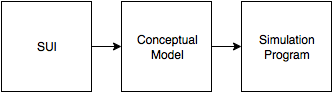
\includegraphics[height=1in,width=3.6in]{sui_mod_sim} 
		\caption{The role of the conceptual model\label{fig:01}} 
	\end{center} 
\end{figure}

\subsection{Objective} \label{sec:model_obj}
For this project, the objective is to model the egress of pedestrians from a stadium (Georgia 
Tech's Bobby Dodd Stadium). The conceptual model must be generated to represent the SUI which is 
the pedestrian movements.

\subsection{Input} \label{sec:model_in}
Model inputs includes pedestrian and map information. The number of pedestrians and their 
characteristics: travel speed and destination. The simulation environment (walkways, destinations, 
etc.) must be input as map information. The map information should be input as a grid (for the CA 
implementation). It must contain definitions of walkways, destinations, stadium exits, and street 
crossings (crossings can be turned on and off).
	
\subsection{Output} \label{sec:model_out}
The model output is the simulated egress of the pedestrians (specified during input) through the 
modeled environment (map information given as an input).	

\subsection{Content} \label{sec:model_cont}
The model does not include activities inside the stadium; however, the stadium exits do 
provided inputs to the simulation. Therefore, the stadium and activities within are regarded as 
exogenous entities for this model. The stadium (Bobby Dodd Stadium) can hold 55,000 spectators 
\cite{Dodd:Misc} which provides an upper limit on the number of spectators to include in the 
simulation. \\

\noindent
The endogenous entities in this model are pedestrians and map objects (walkways, streets, 
etc.). A queuing model is implemented for the pedestrian entities. They are then placed into the 
model as space opens up at exit locations (previous pedestrians walk away). Pedestrian entities 
contain properties for waking speed and selected destination. The walking speed distribution is 
obtained from research in \cite{young1999evaluation} and is similar to that used in 
\cite{burstedde2001simulation}. The walking speeds for each pedestrian are drawn from the normal 
distribution shown in Table \ref{tbl:01} and Figure \ref{fig:speed}.\footnote{The speeds are capped 
at a minimum of 0.153 m/s which is the threshold used in \cite{young1999evaluation}to determine 
walking.}
	
\begin{table}[H]
	\centering
	\caption{Pedestrian Walking Speed Distribution \cite{young1999evaluation}}
	\label{tbl:01}
	\begin{tabular}{l|ll}
		& ft/sec & m/sec \\ \hline
		Mean      & 4.40   & 1.340 \\
		Std. Dev. & 0.87   & 0.265
	\end{tabular}
\end{table}

\begin{figure}[h]
	\begin{center} 
		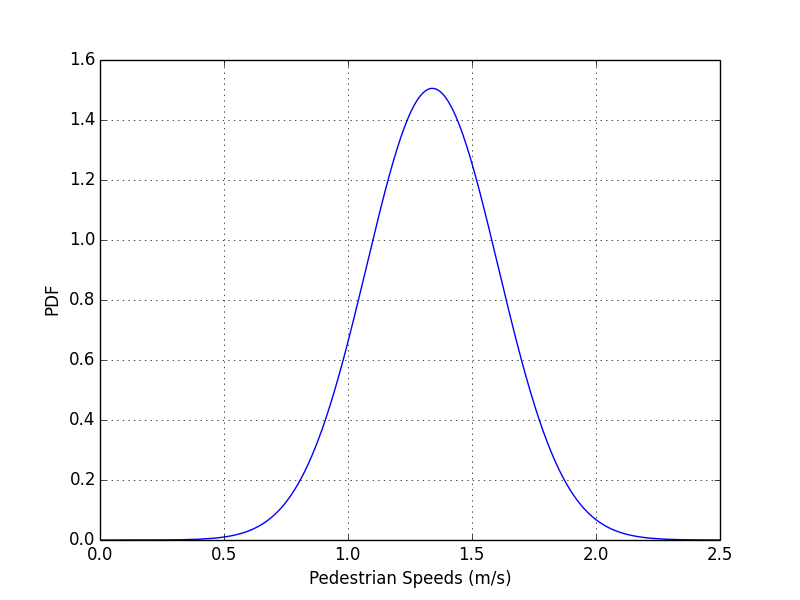
\includegraphics[height=4in,width=5.5in]{speed_dist_pdf} 
		\caption{PDF of Pedestrian Speeds\label{fig:speed}}
	\end{center} 
\end{figure}

\noindent
Map information is represented as a grid of cells that measure $0.25 m^2$ ($0.5 m$ sides). These 
dimensions were chosen as a simplification of that used in \cite{blue2001cellular}. Each cell is 
given a type that represents information relevant to this simulation. More specifically, the cells 
are identified as walkways, crosswalks, streets, or prohibited (no walking allowed).

\subsection{Assumptions and Simplifications} \label{sec:modle_ass}
Pedestrian entities are assumed to always travel toward their predetermined destination (they 
do not change destinations during the simulation) and to stay on the allowed paths. The 
pedestrian model does not include personal attributes, although some attributes may correlate 
with pedestrian walking speed (e.g., age), this is taken into account through the walking speed 
distribution. Additionally, diagonal travel is not modeled. Only movements directly to cells 
that share a side with the current cell are allowed (North, South, East, and West). Further, 
pedestrians are assumed to travel at a constant speed if possible (the pedestrians will travel less 
cells than possible in a time step if something is blocking their route).\\

\noindent
The map information is simplified to a 2-D grid (for use with CA). Terrain attributes (incline, 
material, etc.) are not included. Further, due to the grid architecture, diagonal walkways may only 
be modeled as a stair step of square cells.\\

\noindent
These simplifications/assumptions were made in order to focus on the main part of the simulation 
and get the simulation running within the alloted time. It is fully understood that this type of 
model is very complex and could have much more detail (especially in the area of pedestrian 
intelligence). However, the author is confident that much of the essentials to the model were 
implemented.

%%%%%%%%%%%%%%%%%%%%%%%%%%%%%%%%%%%%%%%%%%%%%%%%%%%%%%%%%%%%%%%%%%%%%%%%%%%%%%%%%%%%%%%%%%%%%%%%
\section{Simulation Development} \label{sec:simdev}
Pedestrian movement is a dynamical system and for this project, pedestrian egress from a 
stadium, it will be modeled as a discrete time dynamical system using CA. The simulation grid 
is made up of cells that are either ``allowed'' or ``prohibited'' for pedestrian traffic. A 
``floor field'' \cite{varas2007cellular} is calculated for each destination and used to 
influence the movement decisions of the pedestrians. The pedestrians enter the simulation at 
the cells designated for the stadium exit(s). A simple time stepping loop (see Algorithm 
\ref{alg:1}) is then used to move the pedestrians to their respective destinations. A high 
level representation of the simulation algorithm is presented below (Algorithm \ref{alg:2}).

\begin{algorithm}[h]
\DontPrintSemicolon
\KwData{Map information, number of pedestrians}
Define distribution of pedestrian speeds\;
Define distribution of pedestrian destinations\;
Create a queue of pedestrian objects\;
Create map object\;
Create separate static fields for each destination\;
\For{number of time steps}{
  	pop pedestrinas off queue and place at stadium exit\;
  	update pedestrian positions\;
  	visualize map\;
}
\caption{High Level Simulation Algorithm \label{alg:2}}
\end{algorithm}

\subsection{Simulation Grid} \label{sec:simgrid}
A simulation grid is created to represent the desired map divided into cells. Each cell has an 
attribute that indicates its type. A cell can have any of the types listed below.
\begin{enumerate}
	\item Prohibited
	\item Walkway
	\item Street
	\item Crossing
	\item Simulation Entry point (also allowed walkway)
	\item Simulation Exit point (also allowed walkway)
\end{enumerate}

\noindent
Using these attributes the simulation will be able to make decisions. If a cell is marked as 
prohibited, pedestrians will not be allowed to move to those locations. Walkways and crossings 
will be allowed. Crossing cells are identified separately so that the simulation can 
periodically open and close the crossing to simulate real life traffic scenarios. The 
simulation will insert and remove pedestrians at entry and exit point cells respectively.\\

\noindent
A ``floor field'' \cite{varas2007cellular} is calculated for each destination by assigning a 
value of 1 to the destination cells and then incrementing the value of neighboring cells for 
each step they are away from the destination. This ``field'' is used to ``force'' pedestrians 
through the grid to their desired destination. The calculation of this field is similar to a 
breadth-first search in graph theory and runs in $O(m+n)$ time (where $n$ is the number of gird 
rows and $m$ is the number of grid columns). Example floor fields for the map simulated are 
presented in Appendix \ref{sec:A:ff}.\\

\noindent
Each ``cell'' object also has attributes for the pedestrian currently occupying the cell. This 
provides information to the movement calculations (state transitions).

\subsection{Pedestrian Objects} \label{sec:simped}
The simulation defines a pedestrian object with the following attributes:
\begin{enumerate}
	\item Coordinates (location on the grid)
	\item Destination ID
	\item Speed (m/s)
\end{enumerate}

\noindent
The pedestrian speeds are drawn from the distribution defined in Section \ref{sec:model} which 
describes the conceptual model. The destination is selected at random from a list of possible 
destinations defined by the map input. All destinations have equal probability of being chosen.

\subsection{Pedestrian Movements (State Transitions)} \label{sec:simmove}
Each time step of the simulation represents 1 second of time. At each time step pedestrians are 
placed at the stadium exits. In order to make the simulation more realistic, the stadium exit cells 
are randomly filled by new pedestrians at the beginning of each time step. This prevents the 
unrealistic situation of a solid wall of pedestrians exiting the stadium at exactly the same time 
walking shoulder to shoulder.
 
\noindent
Once the pedestrian is placed in the simulation grid, the moves are calculated by first calculating 
the distance the pedestrian may move. The distance $d$ (number of cells) a pedestrian can travel 
for a given time step is calculated by Equation \ref{eqn:dist}. Where $s$ is the pedestrian speed, 
$t$ is the loop time step (1 second), and $r_{prev}$ is the remainder of the 
previous distance calculation for the particular pedestrian.

\begin{equation} \label{eqn:dist}
d = \lfloor s*t + r_{prev} \rfloor
\end{equation}

\noindent
A list of possible cells to which the pedestrian may move is then assembled using an algorithm 
similar to a breadth-first-search in graph theory. As the algorithm looks for cells that are within 
the pedestrians movable distance, prohibited cells (including those occupied by another pedestrian) 
are excluded. A move probability $p_m$ is then assigned to each reachable cell using Equation 
\ref{eqn:prob}. Where $U_{current}$ is the floor field potential at the pedestrian's current cell 
and $U_{new}$ is the floor field potential at the reachable cell.

\begin{equation} \label{eqn:prob}
p_m = exp^{U_{current} - U_{new}}
\end{equation}

\noindent
The equation is designed such that lower potentials result in higher probabilities. The cell with 
the highest probability is chosen as the pedestrian's next move. Conflicts (when two or more 
pedestrians pick the same cell) are mitigated by taking the pedestrian that wants it the most 
(highest probability) while the rest select the next cell on their list and the process repeats 
(ties are given to the first pedestrian to pick the cell). The cell currently occupied by the 
pedestrian is left in the list of possibilities so that if no lower potential cells are available 
the pedestrian will stay put (useful for implementing waiting due to traffic signals). In the case 
where a pedestrian is confronted with multiple cells of equal probability, a random choice is made. 
\\

\noindent
Once a pedestrian has reached its destination it is removed from the simulation. The simulation 
terminates once there are no longer any more pedestrians left in the simulation grid.

%%%%%%%%%%%%%%%%%%%%%%%%%%%%%%%%%%%%%%%%%%%%%%%%%%%%%%%%%%%%%%%%%%%%%%%%%%%%%%%%%%%%%%%%%%%%%%%%%%%%
\section{Description of Simulation Software} \label{sec:software}

\subsection{Architecture}
The simulation software was written in Python and is based on the example CA simulation given in 
\cite{SayamaBook}. It consists of a time stepping loop that updates the states of the cells 
(pedestrian locations) similar to that shown in Algorithm \ref{alg:1}. Object Oriented (OO) 
practices are implemented by the software. Objects are used to represent pedestrians, the 
simulation grid, cells in the grid, and the simulation itself.

\subsection{Interfaces}
The code is contained in a single file that can be run via the Python interpreter. The simulation 
requires as inputs the number of pedestrians to create and a path to the map text file (see 
Appendix \ref{sec:A:map}) which is used to create the simulation grid. The simulation was built to 
be very general in that different pedestrian walking scenarios could be simulated simply by 
changing the map file and the desired number of pedestrians. The interface is very simple and 
provides good usability.

%%%%%%%%%%%%%%%%%%%%%%%%%%%%%%%%%%%%%%%%%%%%%%%%%%%%%%%%%%%%%%%%%%%%%%%%%%%%%%%%%%%%%%%%%%%%%%%%%%%%
\section{Simulation Results}
This section details the simulation of pedestrian egress from Georgia Tech's Bobby Dodd stadium. 

\subsection{Simulation Grid}
Due to the fact that author has never seen the stadium in person, map data from the 
Internet\footnote{http://binged.it/1TLWUNr} was utilized for building the representation in the 
simulation grid. A screen shot of the map used to generate the simulation grid is shown in Figure 
\ref{fig:bing} while the simulation grid created from the map is shown in Figure \ref{fig:map}.

\begin{figure}[H]
	\begin{center}
		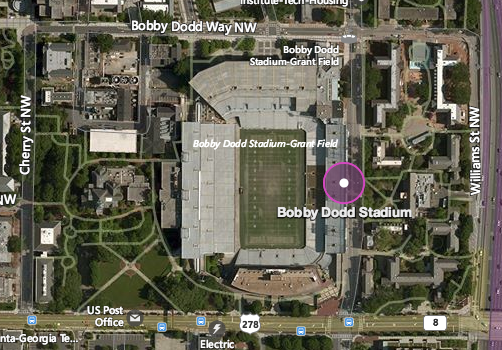
\includegraphics[height=4in,width=5.5in]{stadium_bing_map} 
		\caption{Aerial map of Bobby Dodd stadium and surrounding area.\label{fig:bing}}
	\end{center} 
\end{figure}

\begin{figure}[H]
	\begin{center} 
		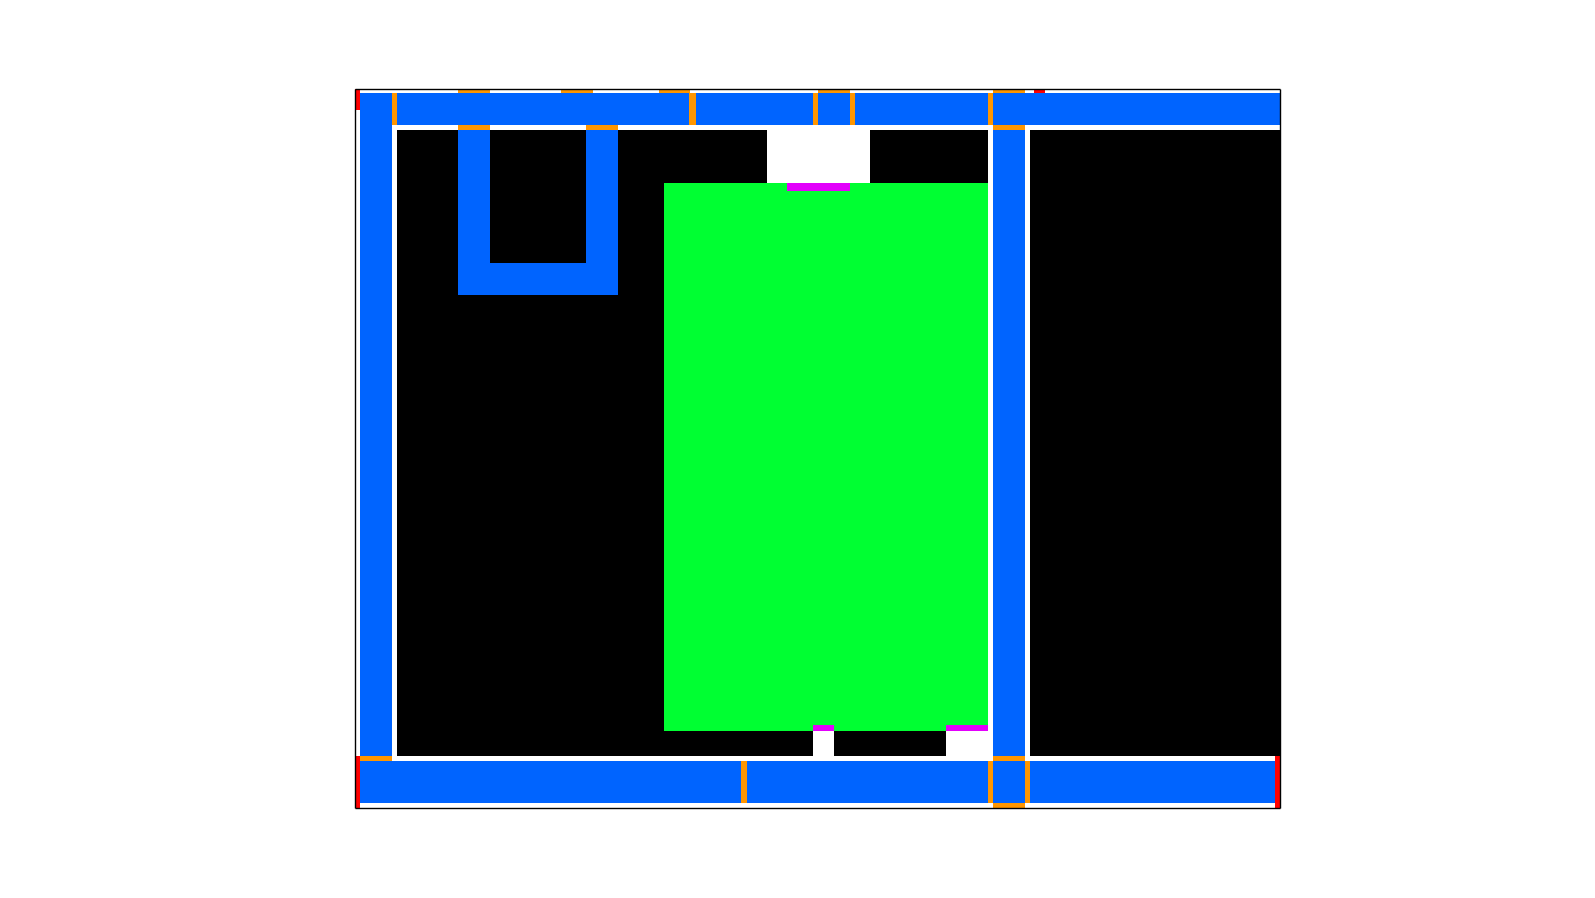
\includegraphics[trim=250 60 220 60, clip, height=4in, width=5.5in]{stadium_simulation_map} 
		\caption{Simplified map of Bobby Dodd stadium and surrounding area implemented in the 
		simulation. Legend: red = exit, purple = stadium exit, white = walkway, orange = crossing, 
		black = prohibited, green = stadium\label{fig:map}}
	\end{center} 
\end{figure}

\noindent
Note the map was substantially simplified in order to get the most relevant data in a reasonable 
amount of time as generating the map file (see the map file used in Appendix \ref{sec:A:map}) was 
significant undertaking.\\

\noindent
As described in Section \ref{sec:simgrid}, the simulation calculated ``floor fields'' for each 
destination. The fields gave lower values to cells closer to the destination. The movement 
calculations utilized these fields (see Section \ref{sec:simmove}). The floor fields for the 
destinations shown in Figure \ref{fig:map} are presented in Appendix \ref{sec:A:ff}.   

\subsection{Pedestrian Queue}
As discussed in Section \ref{sec:model_cont}, the stadium can hold 55,000 spectators. The 
simulation thus generates 55,000 pedestrian objects with random walking speed and destination. The 
destinations are chosen with equal probabilities and the speeds are drawn from the distribution 
discussed in Section \ref{sec:model_cont}. The equal probability of destination selection is 
verifies by the distribution shown in Figure \ref{fig:dest_dist}. Additionally, the correctness of 
the distribution of pedestrian speeds is demonstrated by Figure \ref{fig:speed_dist_sim}. 

\begin{figure}[H]
	\begin{center}
		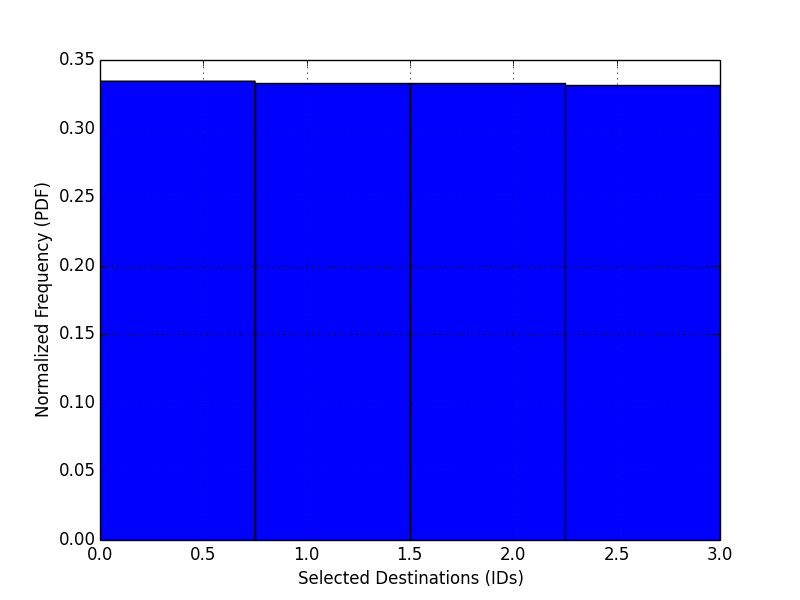
\includegraphics[height=4in,width=5.5in]{destination_dist} 
		\caption{Histogram of pedestrian destination distribution.\label{fig:dest_dist}}
	\end{center} 
\end{figure}

\begin{figure}[H]
	\begin{center} 
		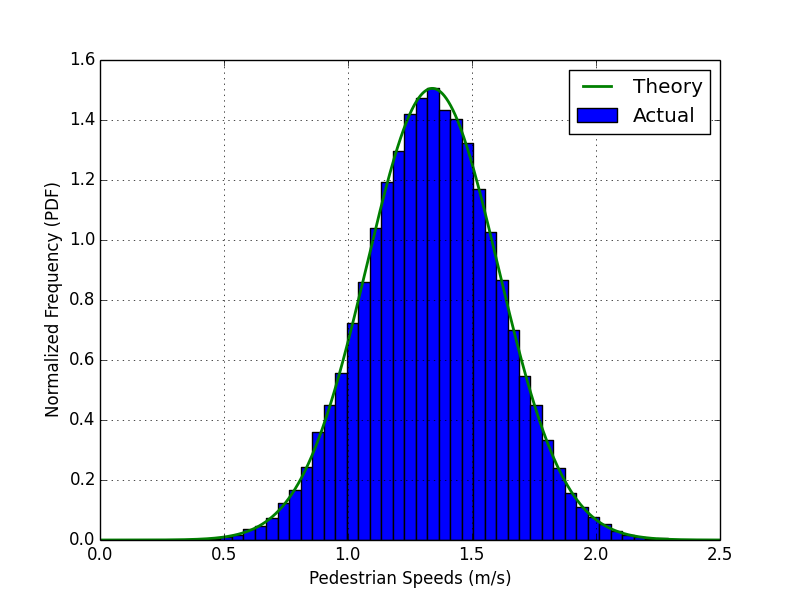
\includegraphics[height=4in, width=5.5in]{speed_dist_hist} 
		\caption{Histogram of pedestrian speeds generated by the 
		simulation.\label{fig:speed_dist_sim}}
	\end{center} 
\end{figure}

\subsection{Simulated Pedestrian Egress}
The figures below show the movement of pedestrians along the map toward their respective 
destinations. Per the project requirements for DL students, the egress from only one exit was 
modeled (the north exit was selected). The animation feature was utilized to verify the performance 
of the simulation was as expected.

\begin{figure}[H]
	\begin{center} 
		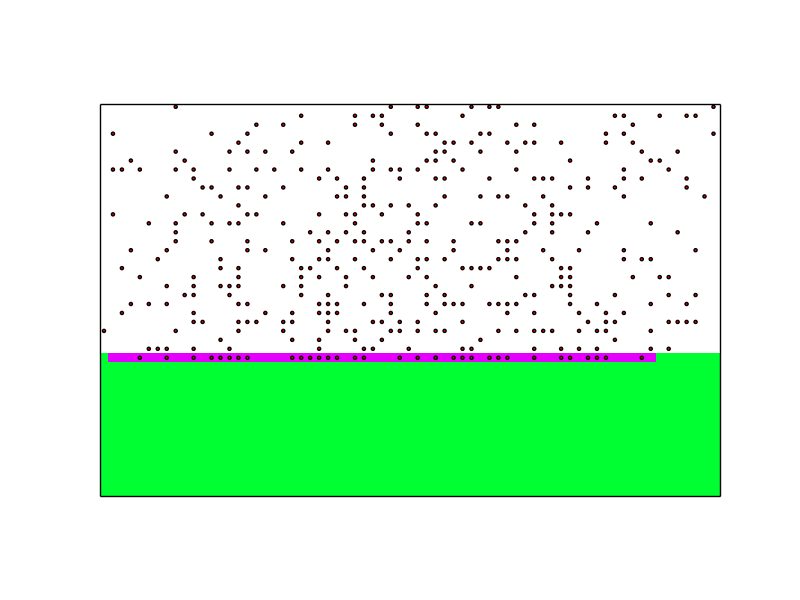
\includegraphics[height=3in,width=4in]{north_exit_zoomed} 
		\caption{Random distribution of pedestrians at North exit.\label{fig:exit_zoomed}}
	\end{center} 
\end{figure}

\begin{figure}[H]
	\begin{center}
		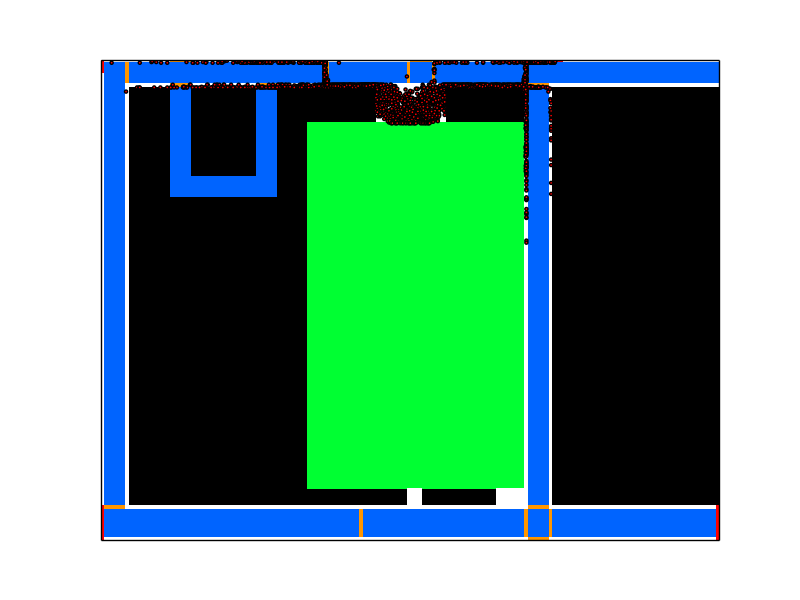
\includegraphics[height=4in,width=5.5in]{sim_100} 
		\caption{Simulation state at 100th time step. Note: The dots representing pedestrians are 
		larger than the grid cells.\label{fig:sim_100}}
	\end{center} 
\end{figure}

\begin{figure}[H]
	\begin{center}
		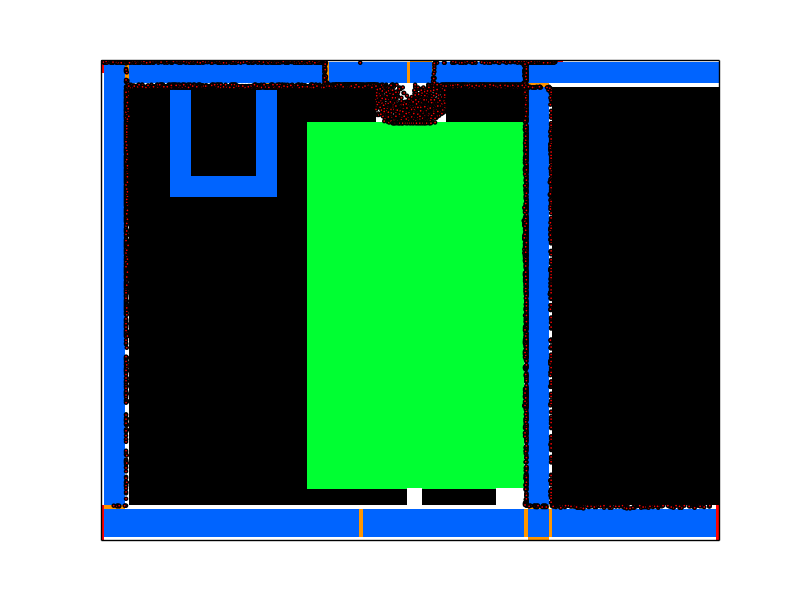
\includegraphics[height=4in,width=5.5in]{sim_300} 
		\caption{Simulation state at 300th time step. Note: The dots representing pedestrians are 
		larger than the grid cells.\label{fig:sim_500}}
	\end{center} 
\end{figure}

\subsection{Egress Timing}
Multiple runs of the simulation were conducted with the results tabulated below in Table 
\ref{tbl:stats}. Each simulation contained 55,000 pedestrian objects; however only one stadium exit 
was modeled (the exit was 60 cells wide). The simulations were run on a MacBook Pro with a 2.4 GHz 
Intel Core 2 Duo processor 
and 4 GB of RAM.

\begin{table}[H]
	\centering
	\caption{Simulation statistics for the egress of 55,000 pedestrian objects from a single, 60 
	cell wide, stadium exit location.}
	\label{tbl:stats}
	\begin{tabular}{|l|l|l|}
		\hline
		               & Average      \\ \hline
		Egress Time    & 49.1 minutes \\ \hline
		Execution Time & 4.63 hours   \\ \hline
	\end{tabular}
\end{table}

\noindent
The simulation times above represent minimum egress times since all street crossings were left open 
(allowing pedestrians to cross streets without waiting). The software currently lacks the ability 
to implement crosswalk signals. As with any modeling and simulation project time constraints 
limited the number of features added to the simulation. Due to the limit resources (in this case 
time) decisions had to be made on feature priority. The crosswalk modeling was put lower on the 
priority list since they are not required to achieve a lower bound on the egress time.\\

\noindent
It is desirable to compare simulated results with actual data for simulation verification. However, 
there was not any such data available to the author (since the author has never actually been to 
Bobby Dodd stadium). However, the author has attended several large sporting events and the 
produced result seems to be within the expected order of magnitude. 

%%%%%%%%%%%%%%%%%%%%%%%%%%%%%%%%%%%%%%%%%%%%%%%%%%%%%%%%%%%%%%%%%%%%%%%%%%%%%%%%%%%%%%%%%%%%%%%%
\section{Summary}
In this report a Cellular Automata (CA) simulation was developed for simulating the egress of 
pedestrians from a stadium. A brief CA background and literature review were presented prior to the 
development of a conceptual model, and simulation software. Code to generate random numbers was 
developed and validated (see Appendix \ref{sec:A:rng}). Finally, pedestrian egress from Georgia 
Tech's Bobby Dodd stadium was simulated and the results presented and validated.\\

\noindent
This project was very challenging but provided a great introduction to the realm of modeling and 
simulation. Due to time constraints, several additional features and updates to the simulator were 
omitted. They are summarized below in Future Work. 

\subsection{Future Work}
There were several features that were not implemented in the software due to time constraints: path 
finding for pedestrians traveling in different directions, more sophisticated pedestrian moves 
(diagonal), and crosswalk signals. Additionally, increases to the simulation speed need to be 
investigated.

\noindent
The conceptual work for crosswalk signaling logic was developed and is presented here for 
reference. Loop through the grid once it is created and generate lists of objects representing sets 
of cells with the same type (stadium exits, destinations, street crossings, etc.). For instance, a 
list of objects representing the crosswalks would be generated (the objects would contain 
information about the location, states of cells, etc.). This would allow for modifying the grid on 
the fly during the simulation. For instance, transient destinations (e.g., bus stop) could be 
simulated by changing the attributes of the destination cells periodically during the simulation.\\

\noindent
As is evident from the results shown in Table \ref{tbl:stats}, the simulations took a very long 
time to run. This indicates speed improvements to the code are desirable before utilizing the 
simulation for large scale research (many simulations). Efforts were made to develop code that ran 
efficiently (estimated $O(n*m)$ running time where $m*n$ are the total number of cells in the 
grid). Never the less, improvements can always be made to software including porting to a compiled 
language (e.g., C/C++) for improved speed.

\subsection{Acknowledgments}
The author would like to acknowledge Mr. Guru Srinagesh for the much appreciated review and 
feedback as well as his willingness to answer many questions during the development of this 
project. 

%%%%%%%%%%%%%%%%%%%%%%%%%%%%%%%%%%%%%%%%%%%%%%%%%%%%%%%%%%%%%%%%%%%%%%%%%%%%%%%%%%%%%%%%%%%%%%%%%%%%
%%% Appendices
\newpage
\begin{appendices}

%%%%%%%%%%%%%%%%%%%%%%%%%%%%%%%%%%%%%%%%%%%%%%%%%%%%%%%%%%%%%%%%%%%%%%%%%%%%%%%%%%%%%%%%%%%%%%%%%%%%
\section{Random Number Generation}\label{sec:A:rng}
As discussed in the main body of this report, the pedestrian simulation utilizes randomness 
in several places. Both uniform and normal distributions were required for the simulation.
Software algorithms have been created for the purpose of generating pseudo random numbers. 
Since the generation is deterministic (software algorithm) the numbers are not truly 
random; however, the algorithms are designed to generate streams of numbers that are not 
correlateable to the previous samples and hence appear random. The Random Number Generators 
(RNGs) implemented are discussed in this appendix.

\subsection{Uniformly Distributed Random Variant}\label{sec:A:rng:uniformrng}
The ``Minimal'' random number generator developed by Park and Miller 
\cite{press1996numerical} was selected to generate a uniform random deviate between 0.0 and 
1.0. The algorithm is presented in \cite{press1996numerical} written in C. It was adapted 
to Python for this project and is presented below.\\

\lstset{language=Python}
\begin{lstlisting}[frame=single, label=some-code, caption=Minimal Random Number Generator]
def min_rand(seed=0):

    # Define constants
    ia = 16807
    im = 2147483647
    am = (1.0/im)
    iq = 127773
    ir = 2836
    mask = 123459876
	
    # Only allow the generator to be seeded once
    if "seed" not in min_rand.__dict__:
        # XORing with MASK allows use of zero and other simple bit patterns
        # for seed.
        min_rand.seed = seed ^ mask

    # Compute idum=(IA*idum) % IM without over-flows by Schrage's method.
    k = min_rand.seed/iq
    min_rand.seed = ia*(min_rand.seed - k*iq) - ir*k
    if min_rand.seed  < 0:
        min_rand.seed += im
    rand_val = am*min_rand.seed  # Convert to a floating result.
    min_rand.seed ^= mask  # Unmask before return.
    
    return rand_val
\end{lstlisting}
\vspace{2mm}

\newpage
\noindent
The generator was tested for the desired behavior using the \emph{Chi-Squared} test 
\cite{Navidi2008Stats} as discussed in class (see equation \ref{eqn:chi2}). 

\begin{equation} \label{eqn:chi2}
A_m = \sum_{i=1}^{k} \frac{O_i - E_i}{E_i}
\end{equation} 

\noindent
Where $O_i$ is the number of values in bin $i$ and $E_i$ is the expected value.
The calculated value of $A_m$ is 27 which is much less than $\chi^*$ of 38.885 for 26 degrees of 
freedom (27 bins) and $\alpha = 0.05$. This indicates acceptable performance of the RNG. The set of 
generated random values used for this test is shown graphically in Figure \ref{fig:A:URNG}.\\

\begin{figure}[H]
	\begin{center} 
		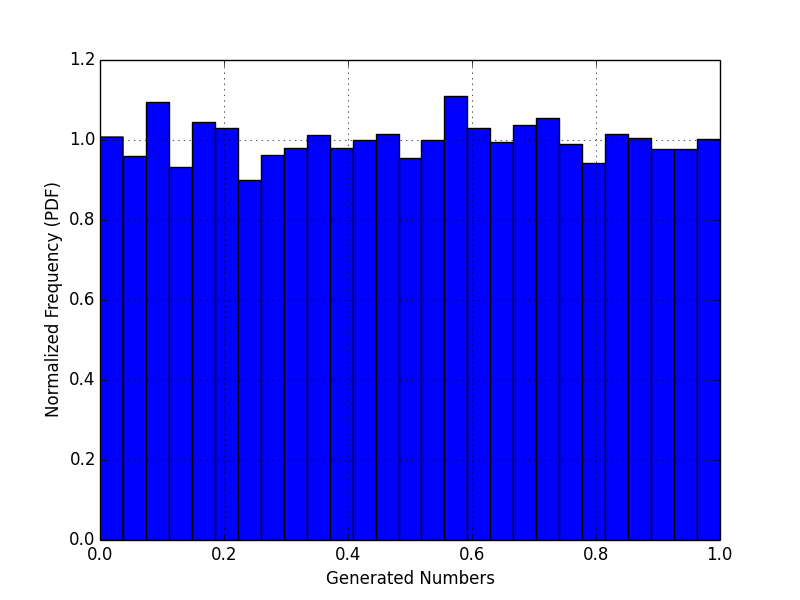
\includegraphics[height=4in,width=5.5in]{uniform_rng} 
		\caption{Histogram of Uniformly Distributed Random Numbers Generated\label{fig:A:URNG}}
	\end{center} 
\end{figure}

\newpage
\subsection{Normally Distributed Random Variant} \label{sec:A:rng:normalmrng}

The \emph{Box-Muller} method \cite{press1996numerical} was selected to generate a normally 
distributed random variate for use in the simulations developed in this report. A similar method 
was also briefly discussed in class.  The algorithm is presented in \cite{press1996numerical} 
written in C. It was adapted to Python for this project and is presented below (note the use of the 
RNG from Section \ref{sec:A:rng:uniformrng}).\\

\begin{lstlisting}[frame=single, label=some-code, caption=Normal Random Number Generator]
def gaussian(mu=0, sigma=1):
# Generate a random number from a Gaussian distribution.
# Adapted from Numerical Recipes in C 2nd ed.

    if 'iset' not in gaussian.__dict__:
        gaussian.iset = 0
    if 'gset' not in gaussian.__dict__:
        gaussian.gset = 0

    if gaussian.iset == 0:
        v1, v2, rsq = 0.0, 0.0, 0.0
        while rsq >= 1.0 or rsq == 0.0:
            v1 = 2.0*min_rand() - 1
            v2 = 2.0*min_rand() - 1
            rsq = v1*v1 + v2*v2
        fac = np.sqrt(-2.0*np.log(rsq)/rsq)
        gaussian.iset = 1
        gaussian.gset = v1*fac
        xi = v2*fac
    else:
        gaussian.iset = 0
        xi = gaussian.gset
     
    # Scale from standard normal distribution to that desired.
    # See page 242 in Statistics for Engineers and Scientists 2nd ed. 
    # by Navidi
    return mu + xi*sigma
\end{lstlisting}
\vspace{4mm}

\noindent
Due to time constraints, the performance of the above algorithm was not verified as throughly as 
the uniform random number generator (presented in Section \ref{sec:A:rng:uniformrng}). However, the 
method is reliable since it was presented in class and in \cite{press1996numerical}. In order to 
ensure the code was written correctly the output was verified visually (see figures below) by 
plotting the theoretical PDF over the normalized histogram (visual goodness of fit test).

\begin{figure}[H]
	\begin{center} 
		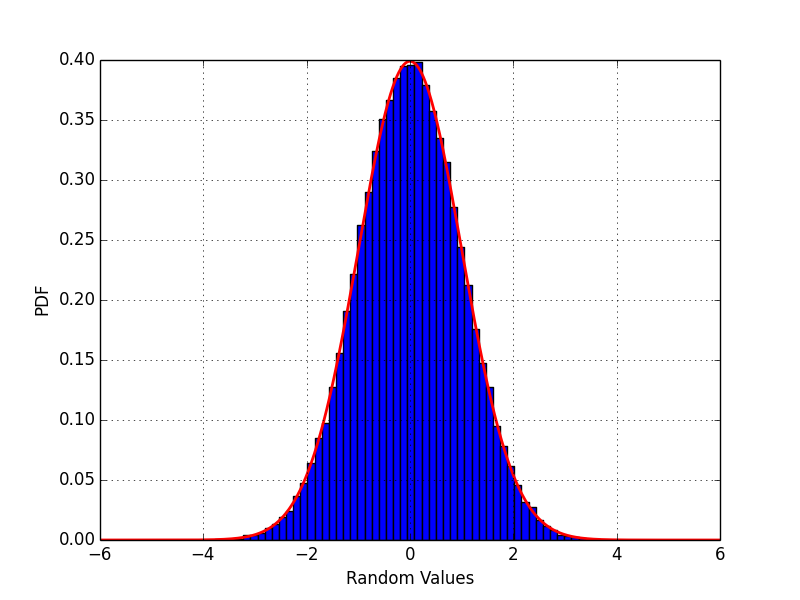
\includegraphics[height=3.3in,width=4.5in]{normal_rng} 
		\caption{Histogram of normally distributed random numbers generated ($\mu = 0$ and 
			$\sigma=1$)\label{fig:A:NRNG}}
	\end{center} 
\end{figure}

\begin{figure}[H]
	\begin{center} 
		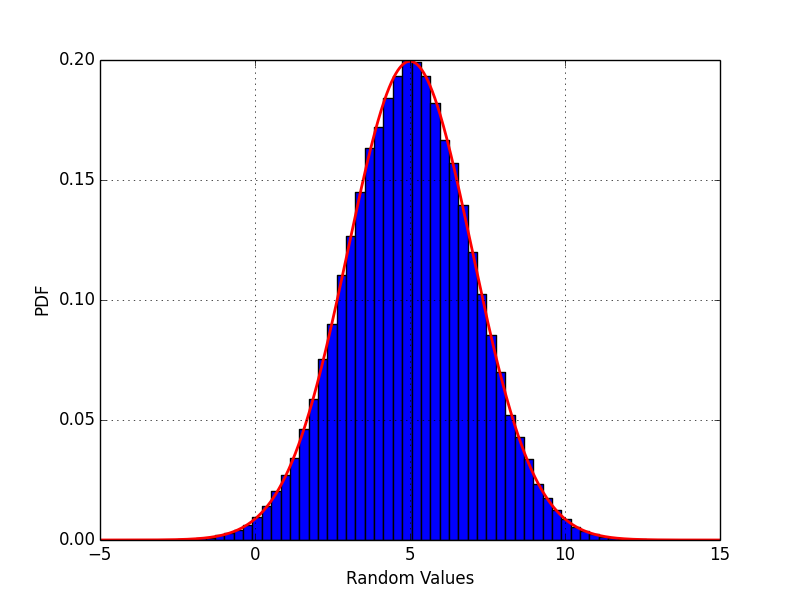
\includegraphics[height=3.3in,width=4.5in]{normal_rng_mu=5_sigma=2} 
		\caption{Histogram of uniformly distributed random numbers generated ($\mu = 5$ and 
		$\sigma=2$)\label{fig:A:NRNG5}}
	\end{center} 
\end{figure}

%%%%%%%%%%%%%%%%%%%%%%%%%%%%%%%%%%%%%%%%%%%%%%%%%%%%%%%%%%%%%%%%%%%%%%%%%%%%%%%%%%%%%%%%%%%%%%%%%%%%
\newpage
\section{Map File Format}\label{sec:A:map}
A custom map file format was developed for getting map information into the simulation. The 
format defines a grid on the first row and then allows blocks of cells to be given a type 
attribute. The simulation assumes any cells not specified to be prohibited. An example map 
file and its corresponding map (from the simulation) are shown below. 

\subsection{Example Map}
\begin{verbatim}
# Test Map File
#
# Grid size (row,col) and size of cell area (arbitrary area unit)
100 100 1
# Define a block (start_row,start_col) to (stop_row,stop_col) of type t
# Cell types:
# 0       = Prohibited (default)
# 1       = Walkway
# 2       = Street
# 4       = Crossing (can also be defined by overlapping 1 and 2)
# 3 to 99 = Arbitrary (for specific use by simulator if needed)
# 1XX     = Destination (can be multiple destinations)
# 2XX     = Starting location (can be multiple starting points)
45 00 50 99 1
00 00 99 05 1
00 48 45 50 1
00 00 02 50 1
00 09 99 19 2
00 60 99 70 2
00 00 00 05 100
00 00 05 00 100
99 00 99 05 101
45 98 50 99 200
\end{verbatim}

\begin{figure}[H]
	\begin{center} 
		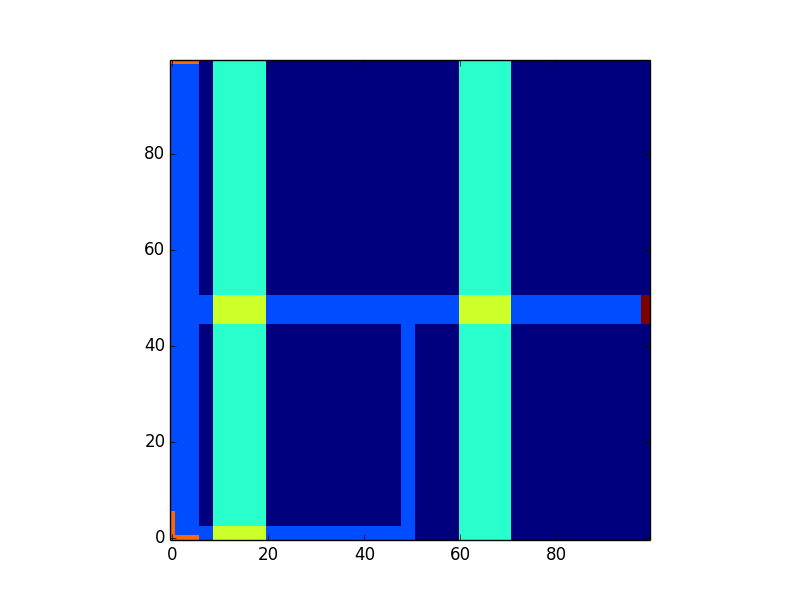
\includegraphics[height=4in,width=5.5in]{map_test_02} 
		\caption{Example map read from data file\label{fig:A:1}} 
	\end{center} 
\end{figure}

\subsection{Bobby Dodd Stadium Map}
\begin{verbatim}
# Grid size (rows, cols) and size of cell area (arbitrary area unit)
700 900 0.5
# Define a block (start_row,start_col) to (stop_row,stop_col) of type t
# Cell types:
# 0       = Prohibited (default)
# 1       = Walkway
# 2       = Street
# 3       = Crossing (can also be defined by overlapping 1 and 2)
# 4 to 5  = Reserved
# 6 to 99 = Arbitrary (for specific use by simulator if needed)
# 1XX     = Destination (can be multiple destinations)
# 2XX     = Starting location (can be multiple starting points)
#
# Walkways
#
50   0  46 899   1 # North sidewalk along North Ave
4   0   0 899   1 # South sidewalk along North Ave
699   0  46   4   1 # West sidewalk along Cherry St
699  36  46  40   1 # East sidewalk along Cherry St
699   0 695 899   1 # North sidewalk along Bobby Dodd Way
663  36 659 899   1 # South sidewalk along Bobby Dodd Way
699 615   0 619   1 # West sidewalk along Techwood Dr
663 651   0 655   1 # East sidewalk along Techwood Dr
658 400 608 500   1 # Walk area at North stadium entrance
75 574  50 614   1 # Walk area at south east stadium entrance
75 445  50 465   1 # South stadium entrance walkway
#
# Streets
#
45   0   5 899   2 # North Ave
694   5  45  35   2 # Cherry St
694   5 664 899   2 # Bobby Dodd Way
699 620   0 650   2 # Techwood Dr
699 100 499 130   2 # Powerplant Dr
529 100 499 255   2 # Powerplant Dr
663 225 499 255   2 # Powerplant Dr
699 450 664 480   2 # Brittain Dr
699 200 690 230   2 # Substation Dr
699 295 690 325   2 # Fowler St
#
# Crossings
#
694 325 664 330 3 # Bobby Dodd Way Crossing at Fowler St
45 375   5 380 3 # North Ave crossing
694 445 664 449 3 # West crossing at Brittian Dr
694 481 664 485 3 # East crossing at Brittian Dr
#
# Destinations
#
699   0 679   4 100 # Side walk opening in north west corner
50   0   0   4 101 # South West corner of map
50 894   0 899 102 # South East corner of map
699 660 695 670 103 # Housing at the North east Corner of the map
#
# Stadium Exits/Entrances
#
# 75 574  75 614 200 # South-East stadium entrance
# 75 445  75 465 201 # South stadium entrance
607 420 607 480 202 # North entrance
#
# Other
#
607 300  75 614   6 # Show Stadium Outline
\end{verbatim}

\begin{figure}[H]
	\begin{center} 
		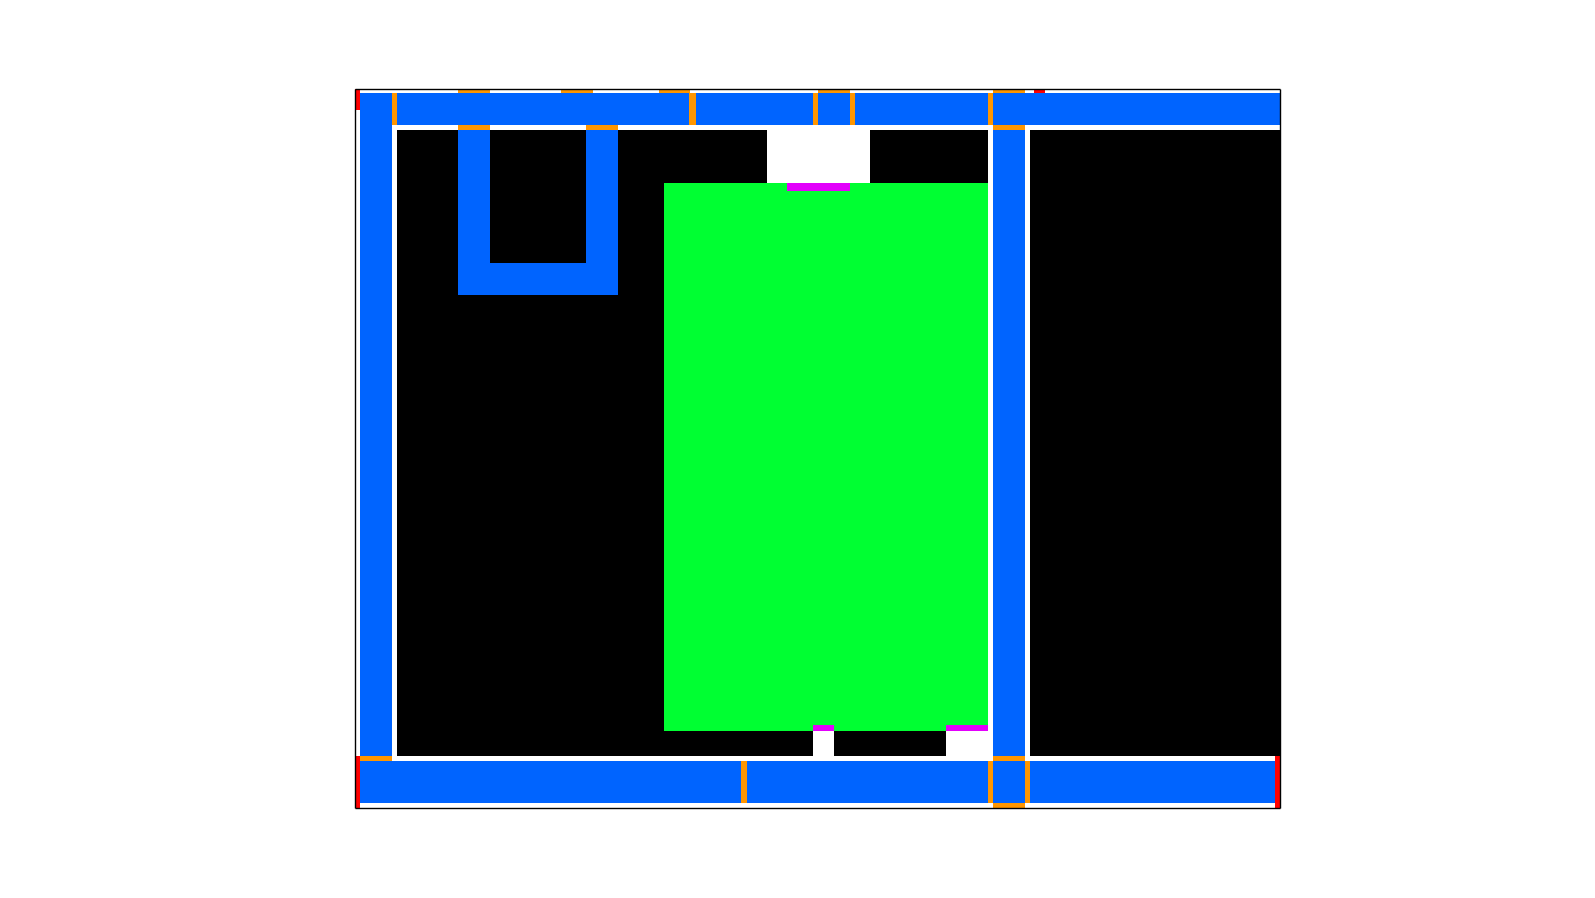
\includegraphics[trim=250 60 220 60, clip, height=4in, width=5.5in]{stadium_simulation_map} 
		\caption{Simplified map of Bobby Dodd stadium and surrounding area implemented in the 
			simulation. Legend: red = exit, purple = stadium exit, white = walkway, orange = 
			crossing, 
			black = prohibited, green = stadium\label{fig:A:map}}
	\end{center} 
\end{figure}

%%%%%%%%%%%%%%%%%%%%%%%%%%%%%%%%%%%%%%%%%%%%%%%%%%%%%%%%%%%%%%%%%%%%%%%%%%%%%%%%%%%%%%%%%%%%%%%%%%%%
\newpage
\section{Floor Fields}\label{sec:A:ff}
A ``floor field'' \cite{varas2007cellular} is calculated for each destination by assigning a 
value of 1 to the destination cells and then incrementing the value of neighboring cells for 
each step they are away from the destination. This ``field'' is used to ``force'' pedestrians 
through the grid to their desired destination. The calculation of this field is similar to a 
breadth-first search in graph theory and runs in $O(m+n)$ time (where $n$ is the number of gird 
rows and $m$ is the number of grid columns). Example floor fields for the map simulated (area 
surrounding GT's Bobby Dodd stadium) are presented below.\\

\begin{figure}[H]
	\begin{center}
		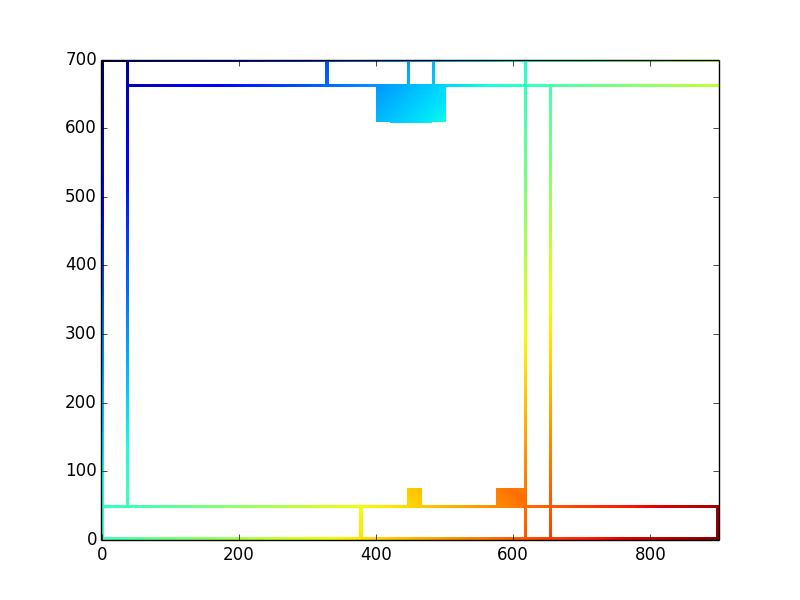
\includegraphics[height=4in,width=5.5in]{floor_field_dest1} 
		\caption{Calculated floor field for destination \#1 
			(sidewalk at North West corner of the map).\label{fig:A:ff1}}
	\end{center} 
\end{figure}

\begin{figure}[H]
	\begin{center}
		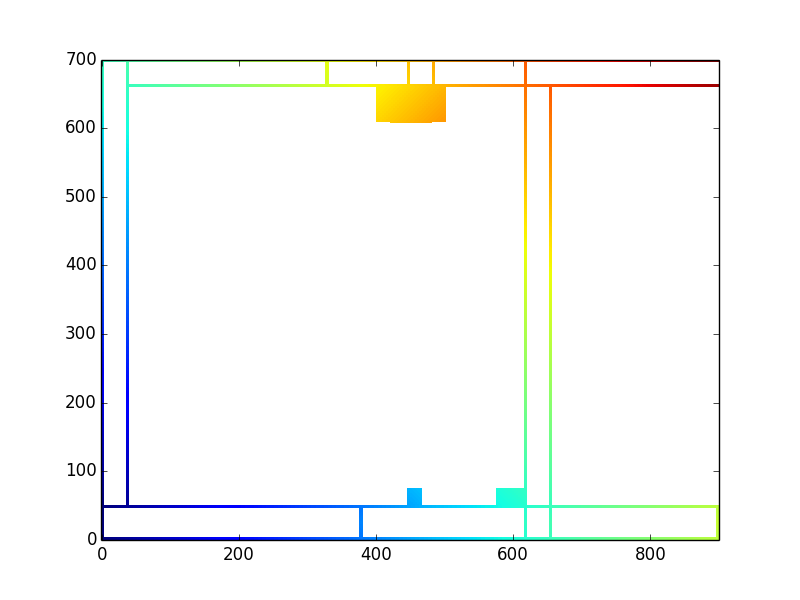
\includegraphics[height=4in,width=5.5in]{floor_field_dest2} 
		\caption{Calculated floor field for destination \#2 
			(South West corner of the map).\label{fig:A:ff2}}
	\end{center} 
\end{figure}

\begin{figure}[H]
	\begin{center}
		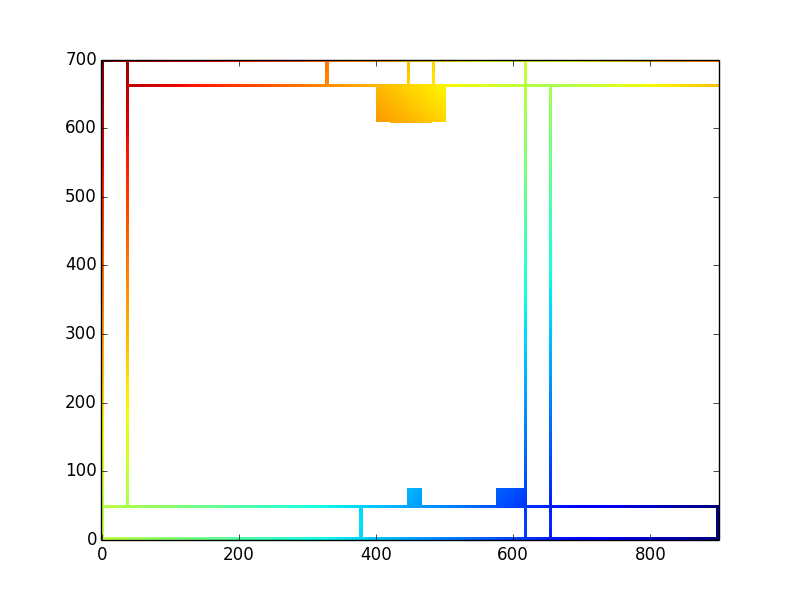
\includegraphics[height=4in,width=5.5in]{floor_field_dest3} 
		\caption{Calculated floor field for destination \#3 
			(South East corner of the map).\label{fig:A:ff3}}
	\end{center} 
\end{figure}

\begin{figure}[H]
	\begin{center}
		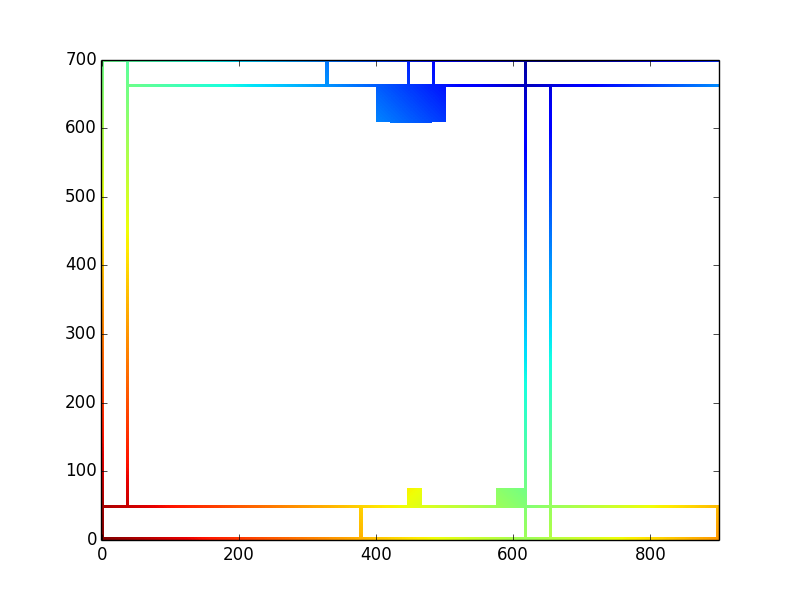
\includegraphics[height=4in,width=5.5in]{floor_field_dest4} 
		\caption{Calculated floor field for destination \#4 
			(student housing at North East corner of the map).\label{fig:A:ff4}}
	\end{center} 
\end{figure}

\end{appendices}  

%%%%%%%%%%%%%%%%%%%%%%%%%%%%%%%%%%%%%%%%%%%%%%%%%%%%%%%%%%%%%%%%%%%%%%%%%%%%%%%%%%%%%%%%%%%%%%%%%%%%
%%% Bibliography
\newpage
\bibliography{cse6730_project1_dcrocker3_report} 
\bibliographystyle{ieeetr}
	
%%%%%%%%%%%%%%%%%%%%%%%%%%%%%%%%%%%%%%%%%%%%%%%%%%%%%%%%%%%%%%%%%%%%%%%%%%%%%%%%%%%%%%%%%%%%%%%%%%%%
%%% End document
\end{document}
